\documentclass[12pt,a4paper]{article}

% ─── Page Layout ───────────────────────────────────────────────────────────────
\usepackage[a4paper, margin=0.8in, headheight=14pt]{geometry}

% ─── Fonts (XeLaTeX) ───────────────────────────────────────────────────────────
\usepackage{fontspec}
\usepackage{unicode-math}
\setmainfont{TeX Gyre Pagella}
\setmonofont[Scale=0.88]{TeX Gyre Cursor}
\setmathfont{Latin Modern Math}

% ─── Packages ──────────────────────────────────────────────────────────────────
\usepackage{xcolor}
\usepackage{colortbl}
\usepackage{titlesec}
\usepackage{enumitem}
\usepackage{tabularx}
\usepackage{booktabs}
\usepackage{array}
\usepackage{amsmath}
\usepackage{tikz}
\usetikzlibrary{shapes.geometric, arrows.meta, positioning, calc, fit, decorations.pathreplacing}
\usepackage{tcolorbox}
\tcbuselibrary{skins, breakable}
\usepackage{hyperref}
\usepackage{fancyhdr}
\usepackage{graphicx}
\usepackage{microtype}
\hyphenpenalty=10000
\exhyphenpenalty=10000
\sloppy
\usepackage{caption}
\usepackage{setspace}
\usepackage{multirow}
\usepackage{tocloft}

% ─── Q&A helper ────────────────────────────────────────────────────────────────
\newcommand{\Q}[1]{\textbf{#1}\par\noindent\ignorespaces}

% ─── Colour Palette ────────────────────────────────────────────────────────────
\definecolor{myred}{RGB}{196,30,58}
\definecolor{mydark}{RGB}{30,30,50}
\definecolor{mygreen}{RGB}{14,120,80}
\definecolor{myteal}{RGB}{0,130,140}
\definecolor{myamber}{RGB}{180,100,0}
\definecolor{mypurple}{RGB}{100,30,160}
\definecolor{mygray}{RGB}{246,247,249}
\definecolor{mgframe}{RGB}{180,185,200}
\definecolor{watermark}{RGB}{145,150,170}
\definecolor{hdrred}{RGB}{250,232,235}
\definecolor{hdrgreen}{RGB}{220,244,233}
\definecolor{hdrteal}{RGB}{220,242,244}
\definecolor{hdramber}{RGB}{253,242,215}
\definecolor{hdrpurple}{RGB}{238,228,255}
\definecolor{hdrgray}{RGB}{238,240,245}
\definecolor{rowalt}{RGB}{250,251,253}

% ─── Section Formatting ────────────────────────────────────────────────────────
\titleformat{\section}
  {\large\bfseries\color{myred}}{\thesection.}{0.5em}{}
  [\vspace{1pt}{\color{myred}\rule{\linewidth}{0.8pt}}]
\titleformat{\subsection}
  {\normalsize\bfseries\color{myteal}}{\thesubsection}{0.5em}{}
\titlespacing*{\section}{0pt}{18pt}{7pt}
\titlespacing*{\subsection}{0pt}{11pt}{4pt}

% ─── Paragraph ─────────────────────────────────────────────────────────────────
\setlength{\parindent}{0pt}
\setlength{\parskip}{4pt}

% ─── TOC Styling ───────────────────────────────────────────────────────────────
\renewcommand{\cfttoctitlefont}{\large\bfseries\color{myred}}
\renewcommand{\cftaftertoctitle}{\par\noindent{\color{myred}\rule{\linewidth}{0.8pt}}}
\setlength{\cftbeforetoctitleskip}{0pt}
\setlength{\cftaftertoctitleskip}{6pt}
\renewcommand{\cftsecfont}{\normalsize\bfseries\color{mydark}}
\renewcommand{\cftsecpagefont}{\normalsize\bfseries\color{mydark}}
\renewcommand{\cftsecleader}{\cftdotfill{\cftdotsep}}
\setlength{\cftbeforesecskip}{7pt}
\renewcommand{\cftsubsecfont}{\small\color{mydark}}
\renewcommand{\cftsubsecpagefont}{\small\color{mydark}}
\setlength{\cftbeforesubsecskip}{3pt}
\setlength{\cftsubsecindent}{1.4em}

% ─── Table helpers ─────────────────────────────────────────────────────────────
\renewcommand{\arraystretch}{1.45}
\setlength{\tabcolsep}{6pt}
\arrayrulecolor{mydark}
\newcolumntype{B}[1]{>{\small\bfseries\raggedright\arraybackslash}m{#1}}
\newcolumntype{Y}{>{\small\raggedright\arraybackslash}X}
\renewcommand{\tabularxcolumn}[1]{m{#1}}

% ─── Header / Footer ───────────────────────────────────────────────────────────
\pagestyle{fancy}
\fancyhf{}
\fancyhead[L]{\small\color{myred}\textbf{PE-EC801A}\;\color{mydark}--- Antennas and Propagation}
\fancyhead[R]{\small\color{myteal}\textbf{Module 4 Notes}}
\fancyfoot[C]{\small\color{mydark}\thepage}
\fancyfoot[R]{\small\color{watermark}\textit{\copyright\ Biraj}}
\renewcommand{\headrulewidth}{0.5pt}
\renewcommand{\footrulewidth}{0.3pt}

% ─── Hyperref ──────────────────────────────────────────────────────────────────
\hypersetup{
  colorlinks=true, linkcolor=myteal, urlcolor=myteal,
  pdfauthor={Biraj Sarkar},
  pdftitle={PE-EC801A --- Module 4 Notes}
}

% ─── tcolorbox styles ──────────────────────────────────────────────────────────
\tcbset{
  tikzbox/.style={
    colback=mygray, colframe=mgframe, boxrule=0.6pt, arc=4pt,
    left=8pt, right=8pt, top=6pt, bottom=6pt,
    colbacktitle=mgframe, coltitle=mydark,
    fonttitle=\small\bfseries
  },
  defbox/.style={
    colback=hdrgreen, colframe=mygreen, boxrule=0.8pt, arc=4pt,
    left=9pt, right=9pt, top=6pt, bottom=6pt,
    colbacktitle=mygreen, coltitle=white,
    fonttitle=\small\bfseries
  },
  formulabox/.style={
    colback=hdrteal, colframe=myteal, boxrule=0.8pt, arc=4pt,
    left=9pt, right=9pt, top=7pt, bottom=7pt,
    colbacktitle=myteal, coltitle=white,
    fonttitle=\small\bfseries
  },
  examplebox/.style={
    colback=hdramber, colframe=myamber, boxrule=0.8pt, arc=4pt,
    left=9pt, right=9pt, top=6pt, bottom=6pt,
    colbacktitle=myamber, coltitle=white,
    fonttitle=\small\bfseries
  },
  masonbox/.style={
    colback=hdrpurple, colframe=mypurple, boxrule=0.8pt, arc=4pt,
    left=9pt, right=9pt, top=6pt, bottom=6pt,
    colbacktitle=mypurple, coltitle=white,
    fonttitle=\small\bfseries
  },
  exambox/.style={
    colback=hdrpurple, colframe=mypurple, boxrule=1pt, arc=5pt,
    left=10pt, right=10pt, top=8pt, bottom=8pt,
    colbacktitle=mypurple, coltitle=white,
    fonttitle=\bfseries,
    breakable, title after break={\textbf{Frequently Asked / Viva Questions (contd.)}}}
}
\tcbset{breakable}

% ─── TikZ styles ───────────────────────────────────────────────────────────────
\tikzset{
  block/.style={rectangle, draw=myteal, fill=hdrteal,
    text width=2.4cm, align=center, minimum height=0.95cm,
    font=\small, rounded corners=3pt, line width=0.7pt},
  redblock/.style={rectangle, draw=myred, fill=hdrred,
    text width=2.4cm, align=center, minimum height=0.95cm,
    font=\small, rounded corners=3pt, line width=0.7pt},
  netnode/.style={rectangle, draw=myteal, fill=hdrteal,
    text width=1.5cm, align=center, minimum height=0.8cm,
    font=\small, rounded corners=3pt, line width=0.7pt},
  sumjunc/.style={circle, draw=myamber, fill=hdramber,
    minimum size=0.62cm, font=\small, line width=0.8pt},
  snode/.style={circle, draw=mypurple, fill=hdrpurple,
    minimum size=0.55cm, font=\footnotesize, line width=0.7pt},
  arrow/.style={-Stealth, thick, color=mydark},
  redarrow/.style={-Stealth, thick, color=myred},
  line/.style={thick, color=mydark}
}

% ═══════════════════════════════════════════════════════════════════════════════
\begin{document}
% ═══════════════════════════════════════════════════════════════════════════════

\begin{center}
  {\LARGE\bfseries\color{myred} PE-EC801A --- Antennas and Propagation}\\[5pt]
  {\normalsize\color{mydark} Semester VIII \quad$\bullet$\quad 3L:0T:0P \quad$\bullet$\quad 3 Credits}\\[3pt]
  {\normalsize\color{myteal}\textbf{Module 4 Exam Notes}}\\[3pt]
  {\small\color{mydark} CGEC \;$|$\; B.Tech ECE (2023--27) \;$|$\; \textit{Biraj Sarkar}}
\end{center}
\vspace{2pt}
\noindent{\color{myred}\rule{\linewidth}{1.5pt}}
\vspace{2pt}

\hypersetup{linkcolor=mydark}
\tableofcontents
\hypersetup{linkcolor=myteal}
\newpage

% ===============================================================================
\section{Yagi-Uda Antenna}
% ===============================================================================

\begin{tcolorbox}[defbox, title={\textbf{Definition of Yagi-Uda Antenna}}]
The \textbf{Yagi-Uda antenna} is a highly directional, narrow-band antenna consisting of a single driven element (usually a half-wave folded dipole) and one or more parasitic elements (a reflector behind it, and directors in front of it) aligned along a central supporting boom.
\end{tcolorbox}

\subsection{Structure and Elements}
The parasitic elements are not connected to the feed line. They receive energy through mutual electromagnetic coupling from the driven element and re-radiate it.

\begin{tcolorbox}[tikzbox, title={Yagi-Uda Antenna Layout}]
\centering
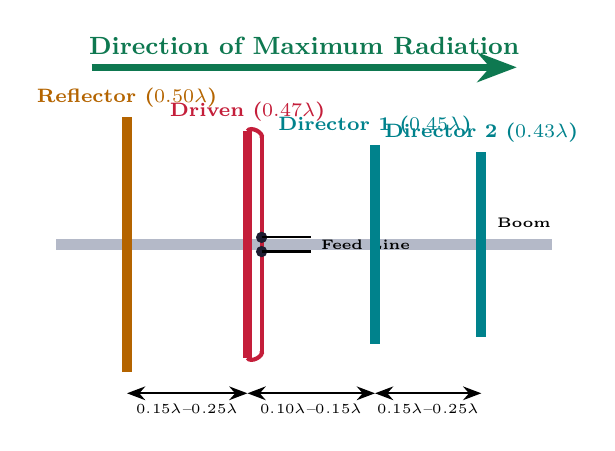
\begin{tikzpicture}[scale=0.9]
  % Supporting Boom
  \draw[line width=4pt, color=mgframe] (-3.5,0) -- (3.5,0);
  \node[above, font=\tiny\bfseries] at (3.1,0.1) {Boom};

  % Reflector
  \draw[line width=3.5pt, color=myamber] (-2.5,-1.8) -- (-2.5,1.8);
  \node[above, font=\scriptsize\bfseries\color{myamber}] at (-2.5,1.8) {Reflector ($0.50\lambda$)};

  % Driven Element (Folded Dipole sketch)
  \draw[line width=3.5pt, color=myred] (-0.8,-1.6) -- (-0.8,1.6);
  \draw[line width=1.5pt, color=myred] (-0.6,-1.5) -- (-0.6,1.5);
  \draw[line width=1.5pt, color=myred] (-0.8,1.6) to[bend left=90] (-0.6,1.5);
  \draw[line width=1.5pt, color=myred] (-0.8,-1.6) to[bend right=90] (-0.6,-1.5);
  \fill[mydark] (-0.6, 0.1) circle (0.08);
  \fill[mydark] (-0.6, -0.1) circle (0.08);
  \draw[thick] (-0.6,0.1) -- (0.1,0.1);
  \draw[thick] (-0.6,-0.1) -- (0.1,-0.1);
  \node[right, font=\tiny\bfseries] at (0.1,0) {Feed Line};
  \node[above, font=\scriptsize\bfseries\color{myred}] at (-0.8,1.6) {Driven ($0.47\lambda$)};

  % Directors
  \draw[line width=3.5pt, color=myteal] (1.0,-1.4) -- (1.0,1.4);
  \node[above, font=\scriptsize\bfseries\color{myteal}] at (1.0,1.4) {Director 1 ($0.45\lambda$)};

  % Director 2
  \draw[line width=3.5pt, color=myteal] (2.5,-1.3) -- (2.5,1.3);
  \node[above, font=\scriptsize\bfseries\color{myteal}] at (2.5,1.3) {Director 2 ($0.43\lambda$)};

  % Spacing dimension lines
  \draw[Stealth-Stealth, thick] (-2.5, -2.1) -- (-0.8, -2.1) node[midway, below, font=\tiny] {$0.15\lambda$–$0.25\lambda$};
  \draw[Stealth-Stealth, thick] (-0.8, -2.1) -- (1.0, -2.1) node[midway, below, font=\tiny] {$0.10\lambda$–$0.15\lambda$};
  \draw[Stealth-Stealth, thick] (1.0, -2.1) -- (2.5, -2.1) node[midway, below, font=\tiny] {$0.15\lambda$–$0.25\lambda$};

  % Radiation Direction Arrow
  \draw[-Stealth, line width=2.5pt, color=mygreen] (-3.0, 2.5) -- (3.0, 2.5) 
    node[midway, above, font=\small\bfseries] {Direction of Maximum Radiation};
\end{tikzpicture}
\end{tcolorbox}

\begin{enumerate}[label=\textbf{\arabic*.}, leftmargin=*, itemsep=4pt]
  \item \textbf{Driven Element:} Typically a folded dipole of resonant length $0.47\lambda$–$0.48\lambda$. The folded dipole structure increases the input impedance from $73\,\Omega$ to around $300\,\Omega$, facilitating impedance matching with standard twin-lead transmission lines.
  \item \textbf{Reflector:} Placed behind the driven element. It is approximately $5\%$ longer than the driven element ($\approx 0.50\lambda$) and spaced $0.15\lambda$–$0.25\lambda$ away. Because it is longer, it is inductive. It redirects the wave in the forward direction.
  \item \textbf{Directors:} Placed in front of the driven element in the direction of the main beam. They are $5\%$ shorter than the driven element ($\approx 0.40\lambda$–$0.45\lambda$) and spaced $0.10\lambda$–$0.30\lambda$ apart. Because they are shorter, they are capacitive, directing wave propagation forward.
\end{enumerate}

\subsection{Characteristics}
\begin{itemize}[leftmargin=*, itemsep=2pt]
  \item \textbf{Directivity/Gain:} Typically $7$–$15\,\text{dB}$ depending on the number of director elements.
  \item \textbf{Bandwidth:} Narrow (typically $2\%$ to $10\%$).
  \item \textbf{Front-to-Back Ratio:} High, meaning it effectively rejects noise from the back.
\end{itemize}

% ===============================================================================
\section{Log-Periodic Antennas}
% ===============================================================================

\begin{tcolorbox}[defbox, title={\textbf{Definition of Log-Periodic Antenna}}]
A \textbf{Log-Periodic Dipole Array (LPDA)} is a multi-element directional antenna designed to operate over an extremely wide bandwidth. Its electrical characteristics (gain, radiation pattern, input impedance) repeat periodically with the logarithm of the frequency.
\end{tcolorbox}

\subsection{Geometric Scaling Laws}
The physical dimensions of the LPDA elements scale according to a geometric progression. Let $L_n$ be the length of the $n$-th dipole element, $d_n$ be the spacing between the $n$-th and $(n+1)$-th elements, and $R_n$ be the distance from the apex to the $n$-th element.

\begin{tcolorbox}[formulabox, title={\textbf{LPDA Scaling Ratios}}]
The geometric scale factor $\tau$ and spacing factor $\sigma$ are defined as:
\[
\tau = \frac{L_{n+1}}{L_n} = \frac{R_{n+1}}{R_n} = \frac{d_{n+1}}{d_n} \quad (0 < \tau < 1)
\]
\[
\sigma = \frac{d_n}{2 L_n}
\]
The apex angle $2\alpha$ of the structure is related to these ratios by:
\[
\tan\alpha = \frac{L_n - L_{n+1}}{2 R_n} = \frac{1 - \tau}{4 \sigma}
\]
\end{tcolorbox}

\begin{tcolorbox}[tikzbox, title={Log-Periodic Dipole Array (LPDA)}]
\centering
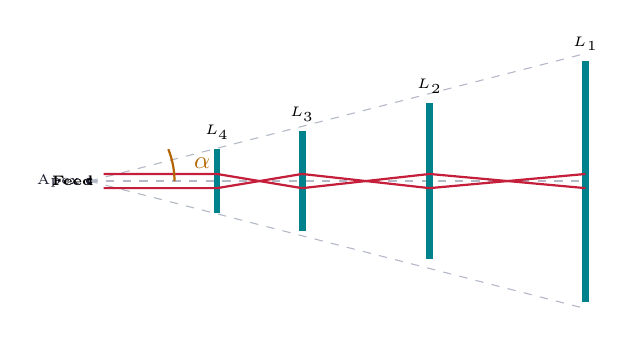
\begin{tikzpicture}[scale=0.9]
  % Apex
  \coordinate (A) at (-4, 0);
  \fill[mydark] (A) circle (0.05) node[left, font=\tiny] {Apex};
  
  % Apex boundaries
  \draw[dashed, color=mgframe] (A) -- (3, 1.8);
  \draw[dashed, color=mgframe] (A) -- (3, -1.8);
  \draw[dashed, color=mgframe] (A) -- (3, 0);

  % Dipoles
  % Element 1 (smallest)
  \draw[line width=2.5pt, color=myteal] (-2.2, -0.45) -- (-2.2, 0.45);
  \node[above, font=\tiny] at (-2.2, 0.45) {$L_4$};
  
  % Element 2
  \draw[line width=2.5pt, color=myteal] (-1.0, -0.7) -- (-1.0, 0.7);
  \node[above, font=\tiny] at (-1.0, 0.7) {$L_3$};
  
  % Element 3
  \draw[line width=2.5pt, color=myteal] (0.8, -1.1) -- (0.8, 1.1);
  \node[above, font=\tiny] at (0.8, 1.1) {$L_2$};
  
  % Element 4 (largest)
  \draw[line width=2.5pt, color=myteal] (3.0, -1.7) -- (3.0, 1.7);
  \node[above, font=\tiny] at (3.0, 1.7) {$L_1$};

  % Crossed feed line
  \draw[thick, color=myred] (-3.8, 0.1) -- (-2.2, 0.1) -- (-1.0, -0.1) -- (0.8, 0.1) -- (3.0, -0.1);
  \draw[thick, color=myred] (-3.8, -0.1) -- (-2.2, -0.1) -- (-1.0, 0.1) -- (0.8, -0.1) -- (3.0, 0.1);
  \node[left, font=\tiny\bfseries] at (-3.8, 0) {Feed};

  % Apex Angle
  \draw[thick, color=myamber] (-2.8,0) arc (0:22:1.2);
  \node[color=myamber, font=\small\bfseries] at (-2.4, 0.25) {$\alpha$};

\end{tikzpicture}
\end{tcolorbox}

\subsection{Principle of Operation (Active Region)}
The feed line is cross-phased between adjacent elements (a $180^\circ$ phase twist). This configuration ensures that at any given frequency:
\begin{itemize}[leftmargin=*, itemsep=3pt]
  \item \textbf{Transmission Region:} Elements that are too short ($L \ll \lambda/2$) present a high capacitive reactance and do not draw much current; they act as a transmission line.
  \item \textbf{Active Region:} Elements whose length is close to half a wavelength ($L \approx \lambda/2$) are resonant. They draw the majority of the current and radiate.
  \item \textbf{Reflective Region:} Elements that are too long ($L \gg \lambda/2$) are highly inductive and act as reflectors.
\end{itemize}
As the operating frequency increases, the active region shifts toward the smaller elements at the apex, maintaining constant beamwidth and input impedance.

% ===============================================================================
\section{Frequency Independent Antennas}
% ===============================================================================

\subsection{Rumsey's Principle}
Rumsey's Principle states that an antenna will be frequency-independent if its physical shape is defined entirely by angles, with no characteristic scale length. If the dimensions are scaled, the antenna looks identical except for a rotation.

\subsection{Examples}
\begin{itemize}[leftmargin=*, itemsep=3pt]
  \item \textbf{Biconical Antenna:} Formed by two co-axial metallic cones with their vertices facing each other. It behaves as a broadband version of a dipole.
  \item \textbf{Equiangular Spiral Antenna:} The boundary curves are defined in polar coordinates by:
  \[
  r = r_0 e^{a\phi}
  \]
  Because the shape is defined purely by exponential growth and angles, it has infinite theoretical bandwidth (practically limited by feed-point dimensions at high frequencies and outer boundaries at low frequencies).
\end{itemize}

\begin{tcolorbox}[tikzbox, title={Biconical Antenna Geometry}]
\centering
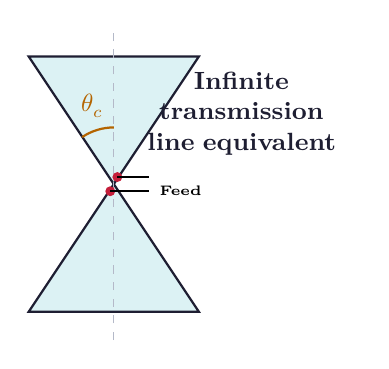
\begin{tikzpicture}[scale=0.9]
  % Top Cone
  \draw[thick, color=mydark, fill=hdrteal] (0,0) -- (-1.2,1.8) -- (1.2,1.8) -- cycle;
  % Bottom Cone
  \draw[thick, color=mydark, fill=hdrteal] (0,0) -- (-1.2,-1.8) -- (1.2,-1.8) -- cycle;

  % Axis
  \draw[dashed, color=mgframe] (0,-2.2) -- (0,2.2);

  % Feed points
  \fill[myred] (0.05, 0.1) circle (0.07);
  \fill[myred] (-0.05, -0.1) circle (0.07);
  \draw[thick] (0.05, 0.1) -- (0.5, 0.1);
  \draw[thick] (-0.05, -0.1) -- (0.5, -0.1) node[right, font=\tiny\bfseries] {Feed};

  % Angle
  \draw[thick, color=myamber] (0,0.8) arc (90:124:0.8);
  \node[color=myamber, font=\small\bfseries] at (-0.3, 1.1) {$\theta_c$};
  \node[font=\small\bfseries\color{mydark}, align=center, text width=2.8cm] at (1.8, 1.0) {Infinite \\ transmission \\ line equivalent};

\end{tikzpicture}
\end{tcolorbox}

% ===============================================================================
\section{Broadcast Antennas}
% ===============================================================================

Broadcast applications require omnidirectional radiation patterns in the horizontal plane to cover a $360^\circ$ service area.

\subsection{Turnstile Antenna}
A \textbf{turnstile antenna} consists of two identical horizontal half-wave dipoles placed perpendicular to each other ($90^\circ$ spatial separation) and excited with a $90^\circ$ phase difference.
\begin{itemize}[leftmargin=*, itemsep=2pt]
  \item The E-field components in the horizontal plane are:
  \[
  E_1 = E_0 \cos\phi, \quad E_2 = E_0 \sin\phi \, e^{j\pi/2} = j E_0 \sin\phi
  \]
  \item The total field is:
  \[
  E_{total} = E_1 + E_2 = E_0 (\cos\phi + j\sin\phi) = E_0 e^{j\phi}
  \]
  \item The magnitude $|E_{total}| = E_0$ is constant, producing a perfectly circular (omnidirectional) radiation pattern in the horizontal plane with circular polarization.
\end{itemize}

\subsection{Vertical Mast Radiators}
For Medium Frequency (MF) AM radio broadcasting, vertical steel towers (mast radiators) of height $H \approx \lambda/4$ or $H \approx 0.583\lambda$ (the anti-fading height, which minimizes sky-wave interference near the ground) are used. The ground acts as a reflector, forming a monopole equivalent.

% ===============================================================================
% MANDATORY QUICK REVISION PAGE
% ===============================================================================
\newpage
\begin{center}
  {\large\bfseries\color{myred} Quick Revision --- Module 4}\\[3pt]
  {\small\color{mydark} Broadband and Broadcast Antennas $|$ PE-EC801A}
\end{center}
\noindent{\color{myred}\rule{\linewidth}{1.2pt}}
\vspace{4pt}

\begin{tcolorbox}[formulabox, title={\textbf{Key Formulas and Metrics at a Glance}}]
\renewcommand{\arraystretch}{1.35}
\begin{tabularx}{\linewidth}{B{5.2cm} X}
LPDA Scale Factor ($\tau$) & $\tau = \frac{L_{n+1}}{L_n} = \frac{R_{n+1}}{R_n} = \frac{d_{n+1}}{d_n} < 1$ \\[4pt]
LPDA Spacing Factor ($\sigma$) & $\sigma = \frac{d_n}{2 L_n}$ \\[4pt]
LPDA Apex Angle ($\alpha$) & $\tan\alpha = \frac{1 - \tau}{4 \sigma}$ \\[4pt]
Log-Spiral Geometry & $r = r_0 e^{a\phi}$ \quad (defined purely by angles) \\[4pt]
Yagi Driven Element Length & $L \approx 0.47\lambda$–$0.48\lambda$ \quad (usually folded dipole) \\[4pt]
Yagi Reflector Length & $L \approx 0.50\lambda$ \quad (inductive, reflects wave forward) \\[4pt]
Yagi Director Length & $L \approx 0.40\lambda$–$0.45\lambda$ \quad (capacitive, steers wave forward) \\
\end{tabularx}
\end{tcolorbox}

\begin{tcolorbox}[defbox, title={\textbf{One-Line Definitions}}]
\begin{itemize}[leftmargin=*, itemsep=2pt, topsep=0pt]
  \item \textbf{Parasitic Element:} An antenna element not electrically connected to the receiver/transmitter, excited via mutual coupling.
  \item \textbf{Folded Dipole:} A dipole antenna with its ends folded back and joined, providing a four-fold increase in input impedance.
  \item \textbf{Active Region:} The zone in a log-periodic array where elements are near resonance ($\approx \lambda/2$) and actively radiating.
  \item \textbf{Rumsey's Principle:} The condition that an antenna shape defined only by angles is frequency-independent.
  \item \textbf{Turnstile Antenna:} An arrangement of two crossed dipoles fed out of phase to produce a circular, omnidirectional horizontal pattern.
  \item \textbf{Anti-Fading Mast:} A vertical tower radiator of height $\approx 0.583\lambda$ that suppresses high-angle sky-wave radiation.
\end{itemize}
\end{tcolorbox}

\begin{tcolorbox}[exambox, title={\textbf{Frequently Asked / Viva Questions}}]
\begin{enumerate}[topsep=0pt, label=\textbf{Q\arabic*.}, itemsep=5pt]
  \item \Q{Explain the operation of parasitic elements in a Yagi-Uda antenna.}
    The reflector (longer than $\lambda/2$) acts inductively, shifting the phase of its re-radiated field to add constructively with the driven element's field in the forward direction. The directors (shorter than $\lambda/2$) act capacitively, shifting the phase to pull the beam forward.
  \item \Q{Why is a folded dipole used as the driven element in a Yagi-Uda antenna?}
    Adding parasitic elements near a dipole severely lowers its input impedance (often down to $<15\,\Omega$), causing mismatch loss. A folded dipole has a high impedance ($300\,\Omega$ in free space), which drops to a convenient $50$–$75\,\Omega$ in the array, making it easy to match to coaxial cables.
  \item \Q{What is the difference between a broadband antenna and a frequency-independent antenna?}
    A broadband antenna operates over a wide range (e.g., Yagi-Uda with $10\%$ bandwidth). A frequency-independent antenna satisfies Rumsey's principle (angular geometry) and has a practically unlimited bandwidth (often $10:1$ or more), as its active zone shifts continuously with frequency.
  \item \Q{How does a Log-Periodic Dipole Array (LPDA) achieve frequency independence?}
    As frequency changes, the "active region" (elements near $\lambda/2$ resonance) moves smoothly along the boom. The active elements scale geometrically, so the antenna's electrical size relative to the operating wavelength remains constant.
  \item \Q{What parameters define the geometry of an LPDA?}
    The geometric scale factor $\tau$ (ratio of adjacent lengths/spacings), the spacing factor $\sigma$ (ratio of spacing to element length), and the apex angle $\alpha$.
  \item \Q{How does a Turnstile antenna produce an omnidirectional pattern in the horizontal plane?}
    It uses two crossed horizontal dipoles fed in phase quadrature ($90^\circ$ phase shift). The resulting fields $E_0\cos\phi$ and $jE_0\sin\phi$ combine vectorially to yield a constant amplitude $|E| = E_0$ at all horizontal angles $\phi$.
  \item \Q{Why is the height of $0.583\lambda$ chosen for AM broadcast mast radiators?}
    At $0.583\lambda$, the antenna produces maximum ground-wave radiation while minimizing high-angle sky-wave radiation. This reduces interference between the ground wave and the ionospheric sky wave, preventing fading in the primary coverage zone.
\end{enumerate}
\end{tcolorbox}

\begin{tcolorbox}[tikzbox, title={Yagi-Uda vs. Log-Periodic Dipole Array (LPDA)}]
\centering
\renewcommand{\arraystretch}{1.55}
{\renewcommand{\arraystretch}{1.55}%
\begin{tabularx}{\linewidth}{|B{3.2cm}|Y|Y|}
\hline
\multicolumn{1}{|>{\centering\arraybackslash}m{3.2cm}|}{\textbf{Parameter}} &
\multicolumn{1}{>{\centering\arraybackslash}Y|}{\textbf{Yagi-Uda Antenna}} &
\multicolumn{1}{>{\centering\arraybackslash}Y|}{\textbf{Log-Periodic (LPDA)}} \\
\hline
Bandwidth & Narrow (typically $2\%$–$10\%$) & Extremely Wide ($10:1$ ratio or more) \\
\hline
Gain & High ($7$–$15\,\text{dB}$ depending on elements) & Moderate ($6$–$10\,\text{dB}$) \\
\hline
Element Design & Parasitic elements of specific lengths & Driven elements of geometrically scaled lengths \\
\hline
Feeder Connection & Driven element only (others mutually coupled) & All elements connected to a cross-phased line \\
\hline
\end{tabularx}}
\end{tcolorbox}

\end{document}
